\documentclass[FinalProj,english,12pt]{ulthese}
  %% Encodage utilisé pour les caractères accentués dans les fichiers
  %% source du document. Les gabarits sont encodés en UTF-8. Inutile avec
  %% XeLaTeX, qui gère Unicode nativement.
  \usepackage[utf8]{inputenc}

  %% Charger ici les autres paquetages nécessaires pour le document.
  %% Quelques exemples; décommenter au besoin.
  \usepackage{amsmath}          % recommandé pour les mathématiques
  \usepackage{icomma}           % gestion de la virgule dans les nombres

  %% Utilisation d'une autre police de caractères pour le document.
  %% - Sous LaTeX
  %\usepackage{mathpazo}         % texte et mathématiques en Palatino
  \usepackage{mathptmx}         % texte et mathématiques en Times

  %% Gestion des hyperliens dans le document. S'assurer que hyperref
  %% est le dernier paquetage chargé.
  \usepackage[hyphens]{url}
  \usepackage{hyperref}
  \hypersetup{colorlinks,allcolors=ULlinkcolor}

  %% Enable multirow in the table
  \usepackage{multirow}

  %% Add the degree symbol among others
  \usepackage{gensymb}

  %% Use multiple equation references
  \usepackage{cleveref}

  %% Style de la bibliographie.
  \bibliographystyle{ieeetr}

  %% Forcing displaystyle for all math in the documento
  \everymath{\displaystyle}

  %% Déclarations de la page titre. Remplacer les éléments entre < >.
  %% Supprimer les caractères < >. Couper un long titre ou un long
  %% sous-titre manuellement avec \\.
  \titre{Indoor soccer pitches lighting design}
  \soustitre{Official 5x5 size indoor soccer pitch with timber floor}
  \auteur{Tiberio Menezes de Oliveira}
  \email{tmoliveira@nyx-hemera.com}
  \univcotutelle{François-Xavier Morin}
  \programme{Lighting course}
  \annee{2015}

\begin{document}

\frontmatter                    % pages liminaires

\pagetitre                      % production de la page titre

\tableofcontents                % production de la TdM
\clearpage

\listoftables                   % production de la liste des tableaux
\clearpage

\listoffigures                  % production de la liste des figures
\clearpage

\mainmatter                     % corps du document

\chapter*{Introduction}
\phantomsection\addcontentsline{toc}{chapter}{Introduction}

This project is regarding the creation of a lighting design for a few interior five-a-side football pitches, also known as futsal. The design herein considers the specifications given by FIFA~\cite{www:fifa_official} and The~FA~\cite{www:the_fa_official} and attempts to respect them at its best. The football pitch's floor is made of timber and it has the official size determined by the FIFA's technical recommendation~\cite{www:fifa_book_spec}. The amount of light is specified by this document~\cite{www:the_fa_guide}, provided by The~FA's website.

The pitches are intended to be rented by private groups of people and it can also host a local competition. Therefore, this facility will be open from $7$AM until $11$PM every day, including during the holidays. People will circulate by foot on the floor, and the space is intended to be used only for futsal matches, even though the size and the required lighting can be shared with other types of gymnasium sports or other type of events. The level light required is $500\: lux$, this is the recommended level to accommodate local competitions and recreational futsal games, according to~\cite{www:the_fa_guide}. The facility's luminaires is used as plain power, because, even though there is some light entering onto the building through the windows, this amount of light is not so significant to be taken into account.

          % introduction
\chapter{Facility Details}

\section{Dimensions}
Based on the technical recommendation provided by FIFA, the official futsal playing pitch dimension should be $40m$ by $20m$. As the pitch is in an indoor facility, the ceiling height should be at least $6.1m$, as defined in~\cite{www:the_fa_guide}.

The facility must have a dimension of $185m \times 53m$ and the height is $8m$, so based on the futsal specification, the height of the ceiling is acceptable. The facility will have eight futsal pitches and the distance between each pitch will be of $3m$. The first and the last pitches will have their side distance between the wall and the pitch of $2m$. The distance from the goal line and the wall will be of $7.5m$. In order to retain the ball within the perimeters of pitch and to avoid disturbance of a concurrent game, a safety soccer net will also be installed between each pitch, the same will be installed behind each goal, which will protect the passages of other players.

The futsal ball has a size number $4$, which means its diameter is around $20cm$, therefore the work plan will be set at $20cm$ because the players have to keep an eye on the ball. Since the ceiling height recommendation is $6.1m$ and the facility's height is $8m$, the luminaires will be suspended at $50cm$ from the ceiling. The Figure~\ref{fig:cavity_dimensions} shows the work plan and the luminaires suspension height.

\begin{figure}[h!]
\centering
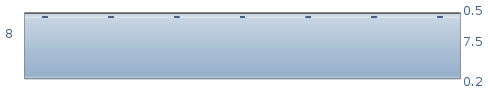
\includegraphics[width=.9\textwidth]{./figs/cavity_dimensions.png}
\caption{Facility's luminaires suspension height and work plan for futsal pitches.}
\label{fig:cavity_dimensions}
\end{figure}

\section{Operations}

The temperature of the facility is maintained between $20\degree$C and $25\degree$C throughout the entire year. This means that the lighting design will not have any corrective factor, thus the variations are very minimal.

During the calculus of the reflection, the floor will be assumed to be dirtier than the wall, because of the accumulated dust and the shoes tracks left by the players. The environment cleanness level is considered moderate because of the missing air filtration system.

Based on the fact gymnasiums commonly have light color walls and ceilings, this facility will follow this specification. For this type of environment the reflectance of the ceiling, wall and floor cavity will be $70\%$, $50\%$ and $20\%$, respectively.

Such as a common facility, the voltage to be utilized in this facility is set at $120V$.

              % chapitre 1
\chapter{Data Comparison}

\section{Table of Comparison}

The Table~\ref{tab:input_data} shows the input data for the entire project.

\begin{table}
\centering
\footnotesize
\begin{tabular}{|l|r|r|r|r|}
  \hline
  \multicolumn{1}{|c|}{\multirow{2}{*}{\textbf{Data to input}}} & \multicolumn{1}{c|}{\multirow{2}{*}{\textbf{Fluorescent}}} & \multicolumn{1}{c|}{\multirow{2}{*}{\textbf{Metal Halide}}} & \multicolumn{1}{c|}{\textbf{High Pressure}} & \multicolumn{1}{c|}{\multirow{2}{*}{\textbf{LED}}} \\
  & & & \multicolumn{1}{c|}{\textbf{Sodium}} & \\
  \hline
  \hline
  \multirow{3}{*}{Catalog} & \multicolumn{1}{c|}{FGB24 6 54T5HO} & \multicolumn{1}{c|}{TH 400M PA22} & \multicolumn{1}{c|}{TH 400S PA22} & \multicolumn{1}{c|}{IBH 30000LM} \\
                           & \multicolumn{1}{c|}{N1D20} & \multicolumn{1}{c|}{SCWA} & \multicolumn{1}{c|}{(LEG 8, SC 1.4)} & \multicolumn{1}{c|}{SD800 MD GZ10} \\
			   & & \multicolumn{1}{c|}{(LEG 8, SC 1.3) }& & \multicolumn{1}{c|}{40K 70CRI} \\
  \hline
  \multirow{3}{*}{Description} & \multicolumn{1}{c|}{spec-beam fluo} & \multicolumn{1}{c|}{open industrial} & \multicolumn{1}{c|}{open industrial} & \multicolumn{1}{c|}{ibeam highbay,} \\
                               & \multicolumn{1}{c|}{highbay, white} & \multicolumn{1}{c|}{highbay, acrylic} & \multicolumn{1}{c|}{highbay, acrylic} & \multicolumn{1}{c|}{30000 lumens,} \\
                               & \multicolumn{1}{c|}{reflector} & \multicolumn{1}{c|}{reflector} & \multicolumn{1}{c|}{reflector} & \multicolumn{1}{c|}{acrylic lens} \\
  \hline
  Survival rate at relamping & 80\% & 80\% & 80\% & 80\% \\
  \hline
  Hours between & \multirow{2}{*}{$24500$} & \multirow{2}{*}{$1400$} & \multirow{2}{*}{$19200$} & \multirow{2}{*}{$60000$} \\
  relamping & & & & \\
  \hline
  Months between & \multirow{2}{*}{$12$} & \multirow{2}{*}{$12$} & \multirow{2}{*}{$12$} & \multirow{2}{*}{$12$} \\
  cleaning & & & & \\
  \hline
  Infrastructure cost & \multirow{2}{*}{$518.00$\$} & \multirow{2}{*}{$518.00$\$} & \multirow{2}{*}{$518.00$\$} & \multirow{2}{*}{$518.00$\$} \\
  per $kW$ of lighting & & & & \\
  \hline
  Electrical energy cost & $0.093$\$ & $0.093$\$ & $0.093$\$ & $0.093$\$ \\
  \hline
  Electrical demand cost & $11.00$\$ & $11.00$\$ & $11.00$\$ & $11.00$\$ \\
  \hline
  Hours of utilization & \multirow{2}{*}{$5840$} & \multirow{2}{*}{$5840$} & \multirow{2}{*}{$5840$} & \multirow{2}{*}{$5840$} \\
  per year & & & & \\
  \hline
  Cost per luminaire: & \multirow{2}{*}{$87.00$\$} & \multirow{2}{*}{$87.00$\$} & \multirow{2}{*}{$87.00$\$} & \multirow{2}{*}{$87.00$\$} \\
  individual relamping & & & & \\
  \hline
  Cost per luminaire: & \multirow{2}{*}{$9.00$\$} & \multirow{2}{*}{$9.00$\$} & \multirow{2}{*}{$9.00$\$} & \multirow{2}{*}{$9.00$\$} \\
  collective relamping & & & & \\
  \hline
  Cost per luminaire: & \multirow{2}{*}{$25.00$\$} & \multirow{2}{*}{$25.00$\$} & \multirow{2}{*}{$25.00$\$} & \multirow{2}{*}{$25.00$\$} \\
  collective cleaning & & & & \\
  \hline
  Facility's length & $53m$ & $53m$ & $53m$ & $53m$ \\
  \hline
  Facility's width & $185m$ & $185m$ & $185m$ & $185m$ \\
  \hline
  Facility's height & $8m$ & $8m$ & $8m$ & $8m$ \\
  \hline
  Desired maintained & \multirow{2}{*}{$500$} & \multirow{2}{*}{$500$} & \multirow{2}{*}{$500$} & \multirow{2}{*}{$500$} \\
  illumination (lux) & & & & \\
  \hline
  Amount of lamps & \multirow{2}{*}{$6$} & \multirow{2}{*}{$1$} & \multirow{2}{*}{$1$} & \multirow{2}{*}{$1$} \\
  per device & & & & \\
  \hline
  Ballast factor & $1.0$ & $1.0$ & $1.0$ & $1,0$ \\
  \hline
  L.D.D. & $0.86$ & $0.86$ & $0.86$ & $0.9$ \\
  \hline
  L.L.D. & $0.78$ & $0.74$ & $0.71$ & $0.99$ \\
  \hline
  L.L.F. & $0.67$ & $0.64$ & $0.61$ & $0.89$ \\
  \hline
  Coefficients of & \multirow{2}{*}{$0.95$} & \multirow{2}{*}{$0.93$} & \multirow{2}{*}{$0.9$} & \multirow{2}{*}{$1.04$} \\
  Utilization & & & & \\
  \hline
  Lumens per lamps & $4450$(rated) & $36000$ & $47500$ & $32911$ \\
  \hline
  Device power & \multirow{2}{*}{$360$} & \multirow{2}{*}{$458$} & \multirow{2}{*}{$465$} & \multirow{2}{*}{$310$} \\
  (lamps + ballast) & & & & \\
  \hline
  Luminaire price & $236.00$\$ & $162.00$\$ & $196.00$\$ & $722.00$\$ \\
  \hline
  Luminaire & \multirow{2}{*}{$127.00$\$} & \multirow{2}{*}{$127.00$\$} & \multirow{2}{*}{$127.00$\$} & \multirow{2}{*}{$127.00$\$} \\
  installation cost & & & & \\
  \hline
  Lamp price & $6.39$\$ & $21.49$\$ & $24.53$\$ & $67.00$\$ \\
  \hline
\end{tabular}
\caption{Input data for each luminaire and lamp.}
\label{tab:input_data}
\end{table}

The Table~\ref{tab:result} shows the results and the costs associated with each type of luminaire.

\begin{table}
\centering
\footnotesize
\begin{tabular}{|l|r|r|r|r|}
  \hline
  \multicolumn{1}{|c|}{\multirow{2}{*}{\textbf{Results}}} & \multicolumn{1}{c|}{\multirow{2}{*}{\textbf{Fluorescent}}} & \multicolumn{1}{c|}{\multirow{2}{*}{\textbf{Metal Halide}}} & \multicolumn{1}{c|}{\textbf{High Pressure}} & \multicolumn{1}{c|}{\multirow{2}{*}{\textbf{LED}}} \\
  & & & \multicolumn{1}{c|}{\textbf{Sodium}} & \\
  \hline
  \hline
  Number of calculated devices & $256$ & $230$ & $188$ & $161$ \\
  \hline
  Number of installed devices & $261$ & $232$ & $189$ & $161$ \\
  \hline
  Number of installed lamps & $1566$ & $232$ & $189$ & $161$ \\
  \hline
  \hline
  Maintained illumination (lux) & $509$ & $504$ & $503$ & $501$ \\
  \hline
  Illuminated surface ($m^2$) & $9805$ & $9805$ & $9805$ & $9805$ \\
  \hline
  Average spacing ($m$) & $6.5$ & $6.5$ & $7$ & $8.25$ \\
  \hline
  Total electric load of & \multirow{2}{*}{$93.96$} & \multirow{2}{*}{$106.256$} & \multirow{2}{*}{$87.885$} & \multirow{2}{*}{$49.91$} \\
  illumination ($kW$) & & & & \\
  \hline
  Power per unit of & \multirow{2}{*}{$9.6$} & \multirow{2}{*}{$10.9$} & \multirow{2}{*}{$9.0$} & \multirow{2}{*}{$5.1$} \\
  area ($W/m^2$) & & & & \\
  \hline
  Average of replaced lamps & \multirow{2}{*}{$449$} & \multirow{2}{*}{$117$} & \multirow{2}{*}{$70$} & \multirow{2}{*}{$20$} \\
  per year & & & & \\
  \hline
  \hline
  Purchase cost of luminaires & $65,596.00$\$ & $37,784.00$\$ & $37,044.00$\$ & $116,242.00$\$ \\
  \hline
  Electric infrastructure cost & $48,671.00$\$ & $55,041.00$\$ & $45,524.00$\$ & $25,853.00$\$ \\
  \hline
  Installation cost of luminaires & $33,147.00$\$ & $29,464.00$\$ & $24,003.00$\$ & $20,447.00$\$ \\
  \hline
  Purchase cost of lamps & $10,007.00$\$ & $4,986.00$\$ & $4,636.00$\$ & $10,787.00$\$ \\
  \hline
  Total investment cost & $153,421.00$\$ & $127,075.00$\$ & $111,207.00$\$ & $173,329.00$\$ \\
  \hline
  \hline
  Annual cost of electricity & $63,469.00$\$ & $71,775.00$\$ & $59,366.00$\$ & $33,714.00$\$ \\
  \hline
  Annual average cost of lamps & $2,869.00$\$ & $2,514.00$\$ & $1,717.00$\$ & $1,340.00$\$ \\
  \hline
  Annual average cost of & \multirow{2}{*}{$7,062.00$\$} & \multirow{2}{*}{$2,613.00$\$} & \multirow{2}{*}{$1,566.00$\$} & \multirow{2}{*}{$492.00$\$} \\
  relamping workforce & & & & \\
  \hline
  Total annual operation cost & $79,925.00$\$ & $82,702.00$\$ & $67,374.00$\$ & $39,571.00$\$ \\
  \hline
\end{tabular}
\caption{Results and costs for each luminaires and lamps.}
\label{tab:result}
\end{table}

              % chapitre 2
\chapter{Recommendations and Common Calculus}

\section{Recommendations}
Based on an analysis of various luminaires available on the market and, taking into account the recommendations from~\cite{www:fifa_light_spec}, a luminaires of high pressure sodium (HPS) would be the best choice. However, if the project is aiming for a long term maintenance, the led luminaires would be considered as the best choice. The initial cost for HPS luminaires is low and its operation cost is not so high, a client seeking the least amount of initial investment will choose the HPS luminaires. In contrast, even though the led luminaires have the higher initial investment cost, on the other hand, have the lowest operation cost, and its economy provided by the low cost operation would pay for the initial investment before its first relamping.

The following luminaires were chosen for this work:
\begin{itemize}
  \item Lithonia IBH 30000LM SD080 MD MVOLT GZ10 40K 70CRI~\cite{www:led_spec}
  \item Lithonia FGB24 6 54T5HO N1D20~\cite{www:fluo_lumin_spec,www:fluo_lamp_spec}
  \item Lithonia TH 400M PA22 SCWA (LEG = 8, SC = 1.3)~\cite{www:mh_hps_lumin_spec,www:mh_lamp_spec}
  \item Lithonia TH 400S PA22 (LEG = 8, SC = 1.4)~\cite{www:mh_hps_lumin_spec,www:hps_lamp_spec}
\end{itemize}
All the luminaires listed are intended to be used in indoor facilities and they can be used in a gymnasium, because of those characteristics all the luminaires could be used for the purpose of this project.

\section{Common Calculus}
\subsection{Cavity Calculus}
In order to calculate the cavity ratio for the project's facility, the Equation~\ref{eq:cavity_ratio} will be used.

\begin{equation}
CR = \frac{5 \times H \times (L + W)}{L \times W}
\label{eq:cavity_ratio}
\end{equation}

The values of $H$, $L$ and $W$ is showed on Figure~\ref{fig:cavity_dimensions}, so the $H$ depends of the cavity that will be calculated, and $L = 53$ and $W = 185$.

In order to calculate the interpolation or extrapolation, the Lagrange theorem for linear interpolation and extrapolation, represented by Equation~\ref{eq:lagrange}, will be used.

\begin{equation}
f(x) = \frac{x_2 - x}{x_2 - x_1} \times y_1 +
       \frac{x - x_1}{x_2 - x_1} \times y_2
\label{eq:lagrange}
\end{equation}

The facility's reflectance cavities are $\rho_c=70\%$, $\rho_w=50\%$ and $\rho_f=20\%$.

\subsubsection{Ceiling Cavity Ratio Calculus}
The value of $H$ for the ceiling cavity ratio ($CCR$) is $0.5m$, and the calculus for $CCR$ is expressed on Equation~\ref{eq:ccr}.

\begin{equation}
\begin{split}
CCR & = \frac{5 \times 0.5 \times (53 + 185)}{53 \times 183} \\
 & = \frac{2.5 \times 238}{9805} \\
 & = 0.061 \\
 & \approx 0.06
\end{split}
\label{eq:ccr}
\end{equation}

\subsubsection{Ceiling Reflectance Calculus}
Using the table for effective ceiling or floor cavity reflectances frr various reflectance combinations, available on the course material of the course, a linear extrapolation using the Equation~\ref{eq:lagrange} will be calculated in order to find the value of the ceiling cavity reflectance ($\rho_{cc}$). The Equation~\ref{eq:reflectance_cc} shows the calculus.

\begin{equation}
\begin{split}
x &= 0.06; \\
x_1 &= 0.2; \\ y_1 &= 67 \\
x_2 &= 0.4; \\ y_2 &= 65
\end{split}
\qquad
\begin{split}
f(x) &= \frac{x_2 - x}{x_2 - x_1} \times y_1 +
       \frac{x - x_1}{x_2 - x_1} \times y_2 \\
 &= \frac{0.4 - 0.06}{0.4 - 0.2} \times 67 +
    \frac{0.06 - 0.2}{0.4 - 0.2} \times 65 \\
 &= \frac{0.34}{0.2} \times 67 -
    \frac{0.14}{0.2} \times 65 \\
 & = 1.7 \times 67 - 0.7 \times 65 \\
 & = 68.4 \\
\rho_{cc} & = 68.4
\end{split}
\label{eq:reflectance_cc}
\end{equation}

\subsubsection{Room Cavity Ratio Calculus}
The value of $H$ for the room cavity ratio ($RCR$) is $7.3m$, and the calculus for $RCR$ is expressed on Equation~\ref{eq:rcr}.

\begin{equation}
\begin{split}
RCR & = \frac{5 \times 7.3 \times (53 + 185)}{53 \times 183} \\
 & = \frac{36.5 \times 238}{9805} \\
 & = 0.886 \\
 & \approx 0.89
\end{split}
\label{eq:rcr}
\end{equation}

\subsubsection{Floor Cavity Ratio Calculus}
The value of $H$ for the floor cavity ratio ($FCR$) is $0.2m$, and the calculus for $FCR$ is expressed on Equation~\ref{eq:fcr}.

\begin{equation}
\begin{split}
FCR & = \frac{5 \times 0.2 \times (53 + 185)}{53 \times 183} \\
 & = \frac{1 \times 238}{9805} \\
 & = 0.024 \\
 & \approx 0.02
\end{split}
\label{eq:fcr}
\end{equation}

\subsubsection{Ceiling Reflectance Calculus}
Using the same table used to find $\rho_{cc}$, a linear interpolation using the Equation~\ref{eq:lagrange} will be made in order to find the value of the floor cavity reflectance ($\rho_{fc}$). The Equation~\ref{eq:reflectance_fc} shows the calculus.

\begin{equation}
\begin{split}
x &= 0.02; \\
x_1 &= 0.2; \\ y_1 &= 20 \\
x_2 &= 0.4; \\ y_2 &= 20
\end{split}
\qquad
\begin{split}
f(x) &= \frac{x_2 - x}{x_2 - x_1} \times y_1 +
       \frac{x - x_1}{x_2 - x_1} \times y_2 \\
 &= \frac{0.4 - 0.02}{0.4 - 0.2} \times 20 +
    \frac{0.02 - 0.2}{0.4 - 0.2} \times 20 \\
 &= \frac{0.38}{0.2} \times 20 -
    \frac{0.18}{0.2} \times 20 \\
 & = 1.9 \times 20 - 0.9 \times 20 \\
 & = 20 \\
\rho_{cc} & = 20
\end{split}
\label{eq:reflectance_fc}
\end{equation}

              % chapitre 3
\chapter{Led Luminaires}

The LED luminaire chosen is a Lithonia IBH 30000LM SD080 MD MVOLT GZ10 40K 70CRI.

\section{Coefficient of Utilization}
The coefficient of utilization ($CU$) is calculated using the table given by the led luminaire~\cite{www:led_photometric}. The calculus is demonstrated by the Equation~\ref{eq:led_cu}.

\begin{equation*}
\begin{split}
\rho_c &= 70\%; \\
\rho_w &= 50\%; \\
\rho_f &= 20\%;
\end{split}
\qquad
\begin{split}
x &= 0.89; \\
x_1 &= 0; \\ y_1 &= 1.16 \\
x_2 &= 1; \\ y_2 &= 1.03
\end{split}
\qquad
\begin{split}
f(x) &= \frac{x_2 - x}{x_2 - x_1} \times y_1 +
       \frac{x - x_1}{x_2 - x_1} \times y_2 \\
 &= \frac{1 - 0.89}{1 - 0} \times 1.16 +
    \frac{0.89 - 0}{1 - 0} \times 1.03 \\
 & = 0.11 \times 1.16 - 0.89 \times 1.03 \\
 & = 1.044 \\
 & \approx 1.04
\end{split}
\label{eq:led_cu_interpol_1}
\end{equation*}

\begin{equation*}
\begin{split}
\rho_c &= 50\%; \\
\rho_w &= 50\%; \\
\rho_f &= 20\%;
\end{split}
\qquad
\begin{split}
x &= 0.89; \\
x_1 &= 0; \\ y_1 &= 1.11 \\
x_2 &= 1; \\ y_2 &= 0.98
\end{split}
\qquad
\begin{split}
f(x) &= \frac{x_2 - x}{x_2 - x_1} \times y_1 +
       \frac{x - x_1}{x_2 - x_1} \times y_2 \\
 &= \frac{1 - 0.89}{1 - 0} \times 1.11 +
    \frac{0.89 - 0}{1 - 0} \times 0.98 \\
 & = 0.11 \times 1.11 - 0.89 \times 0.98 \\
 & = 0.994 \\
 & \approx 0.99
\end{split}
\label{eq:led_cu_interpol_2}
\end{equation*}

\begin{equation}
\begin{split}
\rho_c &= 68.4\%; \\
\rho_w &= 50\%; \\
\rho_f &= 20\%;
\end{split}
\qquad
\begin{split}
x &= 68.4; \\
x_1 &= 50; \\ y_1 &= 0.99 \\
x_2 &= 70; \\ y_2 &= 1.04
\end{split}
\qquad
\begin{split}
f(x) &= \frac{x_2 - x}{x_2 - x_1} \times y_1 +
       \frac{x - x_1}{x_2 - x_1} \times y_2 \\
 &= \frac{70 - 68.4}{70 - 50} \times 0.99 +
    \frac{68.4 - 50}{70 - 50} \times 1.04 \\
 &= \frac{1.6}{20} \times 0.99 +
    \frac{18.4}{20} \times 1.04 \\
 & = 1.036 \\
 & \approx 1.04 \\
CU_{led} & = 1.04
\end{split}
\label{eq:led_cu}
\end{equation}

\section{Light Loss Factor}
The light loss factor ($LLF$) is defined by the Equation~\ref{eq:LLF}.
\begin{equation}
LLF = LLD \times LDD \times BF
\label{eq:LLF}
\end{equation}

\subsection{Lamp Lumen Depreciation}
The Equation~\ref{eq:led_LLD} shows how to calculate the value of the $LLD$.

\begin{equation}
\begin{split}
LLD & = \frac{\text{Total downlight}}{\text{Design/Initial light}} \\
 & = \frac{32,580.5}{32,911} \\
 & =  0.987 \\
 & \approx 0.99
\end{split}
\label{eq:led_LLD}
\end{equation}

\subsection{Luminaire Dirt Depreciation}
Following an operation time of 12 months between cleaning, and taking into account the facility environment with little windows and the use as a gymnasium, the environment, according to the new IES studies for LDD, has a moderate cleaning level. The led luminaire has the following characteristics:
\begin{itemize}
\item Luminaire direct
\item All other class (has an acrylic lens)
\item Class X
\item $LDD = 0.90$, according to the graphic
\end{itemize}

\subsection{Ballast Efficacy}
The led ballast is LEDINTA0700C210DO, and its specification can be found in~\cite{www:led_ballast}. The ballast factor is $1.0$, according to the specification.

\subsection{Calculating the LLF}
The Equation~\ref{eq:led_LLF_calc} shows the calculus of the led's $LLF$.
\begin{equation}
\begin{split}
LLF &= 0.90 \times 0.99 \times 1.0 \\
    &= 0.89
\end{split}
\label{eq:led_LLF_calc}
\end{equation}

\section{Number of Luminaires Calculus}
The amount of luminaires needed to achieve an illuminance of $500$ lux is calculated by the Equation~\ref{eq:led_num_luminaires}.

\begin{equation}
\begin{split}
N_{lum} & = \frac{A_{total\,area} \times L_{Illuminance}}
                {N_{lumens} \times N_{lamps} \times CU \times LLF} \\
 & = \frac{9,805 \times 500}
          {32,911 \times 1 \times 1.04 \times 0.89} \\
 & = \frac{4,902,500}
          {30,496.65} \\
 & = 160.76 \\
 & \approx 161
\end{split}
\label{eq:led_num_luminaires}
\end{equation}

The amount of luminaires to install is $161$, which gives a distribution of $23 \times 7$ and the spacing is calculated by the Equation~\ref{eq:led_spacing}

\begin{equation}
\begin{split}
L: & \frac{185}
          {23} = 8.04\\
W: & \frac{53}
          {7} = 7.57
\end{split}
\qquad
\begin{split}
a & = 8.25 m \\
b & = 1.75 m \\
c & = 8 m \\
d & = 2.5m
\end{split}
\label{eq:led_spacing}
\end{equation}

The illuminance to be maintained for the installed luminaires is calculated by the Equation~\ref{eq:led_maint_light}

\begin{equation}
\begin{split}
L_{Illuminance} & =
\frac {N_{lum} \times N_{lumens} \times N_{lamps} \times CU \times LLF}
      {A_{total\,area}} \\
 & = \frac{161 \times 32,911 \times 1 \times 1.04 \times 0.89}
          {9,805} \\
 & = 500.76 \\
 & \approx 501
\end{split}
\label{eq:led_maint_light}
\end{equation}

\subsection{Checking the Spacing}
The Equation~\ref{eq:led_shr} shows the calculus to check the spacing height ratio ($SHR$) attends the spacing criterion ($SC$).

\begin{equation}
\begin{split}
SHR & = \frac {1}{HM} \times \sqrt{\frac{A_{total\,area}}{N_{lum}}} \\
 & = \frac {1}{7.5} \times \sqrt{\frac{9,805}{161}} \\
 & = 0.133 \times \sqrt{60.9} \\
 & = 0.133 \times 7.8 \\
 & = 1.041 \\
 & \approx 1.04
\end{split}
\label{eq:led_shr}
\end{equation}

The $SC$ given by the led luminaire~\cite{www:led_photometric} is $1.24$ and the $SHR$ has an acceptable value when $SHR \leq SC$, thus the obtained $SHR$ is good.

\section{Luminaires Distribution}
The distribution of the luminaires is represented on Figure~\ref{fig:led_dist}.
\begin{figure}[h!]
\centering
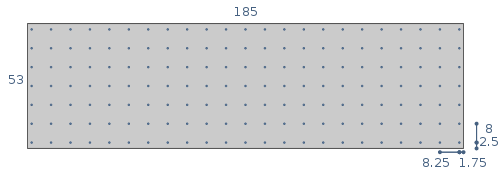
\includegraphics[width=.9\textwidth]{./figs/led_dist.png}
\caption{Led luminaires distributed along the facility ceiling.}
\label{fig:led_dist}
\end{figure}


\section{Calculus of Economy}

\subsection{Energy Consumption}
To calculate the energy consumption, the following data are needed:
\begin{itemize}
\item Number of luminaires: $161$
\item Energy cost: $0.093$\$
\item Electric demand cost: $11.00$\$
\item Number of hours per year: $16 \times 365.25 = 5,844$
\item Luminaire power: $310 W$
\end{itemize}
The numbers of hours per year assumes the leap year, so, the multiplier is $365.25$. The energy consumption results are showed as follow:
\begin{itemize}
\item Total power ($kW$): $161 \times 310 = 49,910 W = 49.91 kW$
\item Total electric demand cost per year: $11 \times 12 \times 49.91 = 6,588.12$\$
\item Total electric consumption cost per year: $5,844 \times 0.093 \times 49.91 = 27,125.69$\$
\item Total energy cost: $33,713.81$\$
\end{itemize}

\subsection{Average of Replaced Lamps per Year}
In order to calculate the average of lamps replaced per year, the following data are needed:
\begin{itemize}
\item Number of luminaires: $161$
\item Number of hours per year: $5,844$
\item Lamp lifetime hours at $80\%$ of survival: $60,000$
\end{itemize}

The Equation~\ref{eq:led_relamp_average} shows the replaced lamps calculus.

\begin{equation}
\begin{split}
 & \text{Individual replaced lamps} \\
M_{individual} & = 20\% \times 161 \times \frac{5,844}{60,000} \\
 & = 3.14 \\
 & \approx 4
\end{split}
\begin{split}
 & \text{Collective replaced lamps} \\
M_{collective} & = 161 \times \frac {5,844}{60,000} \\
 & = 15.68 \\
 & \approx 16
\end{split}
\label{eq:led_relamp_average}
\end{equation}
Taking into account the worst case scenario, the calculation for this average is ceiling rounded. Thus, the average of replaced lamps per year is $20$.

\subsection{Relamping Workforce Cost per Year}
In order to calculate the cost for the relamping workforce per year, the following data are needed:
\begin{itemize}
\item Average of individual lamps replaced per year: $4$
\item Individual relamping cost: $87.00$\$
\item Average of collective lamps replaced per year: $16$
\item Collective relamping cost: $9.00$\$
\end{itemize}
The average cost per year for the collective relamping is $144.00$\$ and for the individual relamping is $348,00$\$, so the total is $492,00$\$


              % chapitre 4
\chapter{Fluorescent Luminaires}

The fluorescent luminaires chosen is FGB24 6 54T5HO N1D20.

\section{Coefficient of Utilization}
The coefficient of utilization ($CU$) is calculated using the table given by the fluorescent luminaire~\cite{www:fluo_photometric}. The calculus is demonstrated by the Equation~\ref{eq:fluo_cu}.

\begin{equation*}
\begin{split}
\rho_c &= 70\%; \\
\rho_w &= 50\%; \\
\rho_f &= 20\%;
\end{split}
\qquad
\begin{split}
x &= 0.89; \\
x_1 &= 0; \\ y_1 &= 1.05 \\
x_2 &= 1; \\ y_2 &= 0.95
\end{split}
\qquad
\begin{split}
f(x) &= \frac{x_2 - x}{x_2 - x_1} \times y_1 +
       \frac{x - x_1}{x_2 - x_1} \times y_2 \\
 &= \frac{1 - 0.89}{1 - 0} \times 1.05 +
    \frac{0.89 - 0}{1 - 0} \times 0.95 \\
 & = 0.11 \times 1.05 - 0.89 \times 0.95 \\
 & = 0.961 \\
 & \approx 0.96
\end{split}
\label{eq:fluo_cu_interpol_1}
\end{equation*}

\begin{equation*}
\begin{split}
\rho_c &= 50\%; \\
\rho_w &= 50\%; \\
\rho_f &= 20\%;
\end{split}
\qquad
\begin{split}
x &= 0.89; \\
x_1 &= 0; \\ y_1 &= 0.99 \\
x_2 &= 1; \\ y_2 &= 0.87
\end{split}
\qquad
\begin{split}
f(x) &= \frac{x_2 - x}{x_2 - x_1} \times y_1 +
       \frac{x - x_1}{x_2 - x_1} \times y_2 \\
 &= \frac{1 - 0.89}{1 - 0} \times 0.99 +
    \frac{0.89 - 0}{1 - 0} \times 0.87 \\
 & = 0.11 \times 0.99 - 0.89 \times 0.87 \\
 & = 0.883 \\
 & \approx 0.88
\end{split}
\label{eq:fluo_cu_interpol_2}
\end{equation*}

\begin{equation}
\begin{split}
\rho_c &= 68.4\%; \\
\rho_w &= 50\%; \\
\rho_f &= 20\%;
\end{split}
\qquad
\begin{split}
x &= 68.4; \\
x_1 &= 50; \\ y_1 &= 0.88 \\
x_2 &= 70; \\ y_2 &= 0.96
\end{split}
\qquad
\begin{split}
f(x) &= \frac{x_2 - x}{x_2 - x_1} \times y_1 +
       \frac{x - x_1}{x_2 - x_1} \times y_2 \\
 &= \frac{70 - 68.4}{70 - 50} \times 0.88 +
    \frac{68.4 - 50}{70 - 50} \times 0.96 \\
 &= \frac{1.6}{20} \times 0.88 +
    \frac{18.4}{20} \times 0.96 \\
 & = 0.954 \\
 & \approx 0.95 \\
CU_{fluo} & = 0.95
\end{split}
\label{eq:fluo_cu}
\end{equation}

\section{Light Loss Factor}
The light loss factor ($LLF$) is defined by the Equation~\ref{eq:LLF}.

\subsection{Lamp Lumen Depreciation}
The Equation~\ref{eq:fluo_LLD} shows how to calculate the value of the $LLD$.

\begin{equation}
\begin{split}
LLD & = \frac{\text{Total downlight}}{\text{Design/Initial light}} \\
 & = \frac{23,382.7}{6 \times 5,000} \\
 & =  0.779 \\
 & \approx 0.78
\end{split}
\label{eq:fluo_LLD}
\end{equation}

\subsection{Luminaire Dirt Depreciation}
Following an operation time of 12 months between cleaning, and taking into account the facility environment with little windows and the use as a gymnasium, the environment, according to the new IES studies for LDD, has a moderate cleaning level. The fluorescent luminaire has the following characteristics:
\begin{itemize}
\item Luminaire direct
\item Open class
\item Class XY
\item $LDD = 0.86$, according to the LDD factor graphic
\end{itemize}

\subsection{Ballast Efficacy}
The fluorescent ballast is ICN-2S54-90C-T@120, and its specification can be found in~\cite{www:fluo_ballast}. The ballast factor is $1.0$, according to the specification.

\subsection{Calculating the LLF}
The Equation~\ref{eq:fluo_LLF_calc} shows the calculus of the fluorescent's $LLF$.
\begin{equation}
\begin{split}
LLF &= 0.86 \times 0.78 \times 1.0 \\
    &= 0.67
\end{split}
\label{eq:fluo_LLF_calc}
\end{equation}

\section{Number of Luminaires Calculus}
The amount of luminaires needed to achieve an illuminance of $500$ lux is calculated by the Equation~\ref{eq:fluo_num_luminaires}.

\begin{equation}
\begin{split}
N_{lum} & = \frac{A_{total\,area} \times L_{Illuminance}}
                {N_{lumens} \times N_{lamps} \times CU \times LLF} \\
 & = \frac{9,805 \times 500}
          {5,000 \times 6 \times 0.95 \times 0.67} \\
 & = \frac{4,902,500}
          {19,117.8} \\
 & = 256.44 \\
 & \approx 256
\end{split}
\label{eq:fluo_num_luminaires}
\end{equation}

The amount of luminaires to install is $261$, which gives a distribution of $29 \times 9$ and the spacing is calculated by the Equation~\ref{eq:fluo_spacing}

\begin{equation}
\begin{split}
L: & \frac{185}
          {29} = 6.38\\
W: & \frac{53}
          {9} = 5.89
\end{split}
\qquad
\begin{split}
a & = 6.5 m \\
b & = 1.5 m \\
c & = 6 m \\
d & = 2.5m
\end{split}
\label{eq:fluo_spacing}
\end{equation}

The illuminance to be maintained for the installed luminaires is calculated by the Equation~\ref{eq:fluo_maint_light}

\begin{equation}
\begin{split}
L_{Illuminance} & =
\frac {N_{lum} \times N_{lumens} \times N_{lamps} \times CU \times LLF}
      {A_{total\,area}} \\
 & = \frac{256 \times 5,000 \times 6 \times 0.95 \times 0.67}
          {9,805} \\
 & = 508.9 \\
 & \approx 509
\end{split}
\label{eq:fluo_maint_light}
\end{equation}

\subsection{Checking the Spacing}
The Equation~\ref{eq:fluo_shr} shows the calculus to check the spacing height ratio ($SHR$) attends the spacing criterion ($SC$).

\begin{equation}
\begin{split}
SHR & = \frac {1}{HM} \times \sqrt{\frac{A_{total\,area}}{N_{lum}}} \\
 & = \frac {1}{7.5} \times \sqrt{\frac{9,805}{261}} \\
 & = 0.133 \times \sqrt{37.57} \\
 & = 0.133 \times 6.13 \\
 & = 0.817 \\
 & \approx 0.82
\end{split}
\label{eq:fluo_shr}
\end{equation}

The $SC$ given by the fluorescent luminaire~\cite{www:fluo_photometric} is $1.29$ and the $SHR$ has an acceptable value when $SHR \leq SC$, thus the obtained $SHR$ is good.

\section{Luminaires Distribution}
The distribution of the luminaires is represented on Figure~\ref{fig:fluo_dist}.
\begin{figure}[h!]
\centering
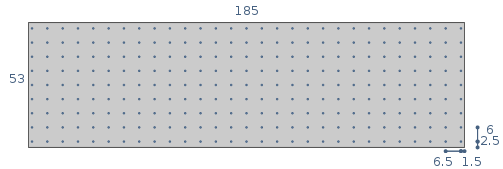
\includegraphics[width=.9\textwidth]{./figs/fluo_dist.png}
\caption{Fluorescent luminaires distributed along the facility ceiling.}
\label{fig:fluo_dist}
\end{figure}

\section{Calculus of Economy}

\subsection{Energy Consumption}
To calculate the energy consumption, the following data are needed:
\begin{itemize}
\item Number of luminaires: $261$
\item Energy cost: $0.093$\$
\item Electric demand cost: $11.00$\$
\item Number of hours per year: $16 \times 365.25 = 5,844$
\item Luminaire power: $360 W$
\end{itemize}
The numbers of hours per year assumes the leap year, so, the multiplier is $365.25$. The energy consumption results are showed as follow:
\begin{itemize}
\item Total power ($kW$): $261 \times 360 = 93,960 W = 93.96 kW$
\item Total electric demand cost per year: $11 \times 12 \times 93.96 = 12,402.72$\$
\item Total electric consumption cost per year: $5,844 \times 0.093 \times 93.96 = 51,066.51$\$
\item Total energy cost: $63,469.23$\$
\end{itemize}

\subsection{Average of Replaced Lamps per Year}
In order to calculate the average of lamps replaced per year, the following data are needed:
\begin{itemize}
\item Number of luminaires: $261$
\item Number of lamps: $6 \times 261 = 1,566$
\item Number of hours per year: $5,844$
\item Lamp lifetime hours at $80\%$ of survival: $24,500$
\end{itemize}

The Equation~\ref{eq:fluo_relamp_average} shows the replaced lamps calculus.

\begin{equation}
\begin{split}
 & \text{Individual replaced lamps} \\
M_{individual} & = 20\% \times 1,566 \times \frac{5,844}{24,500} \\
 & = 74.71 \\
 & \approx 75
\end{split}
\begin{split}
 & \text{Collective replaced lamps} \\
M_{collective} & = 1,566 \times \frac {5,844}{24,500} \\
 & = 373.54 \\
 & \approx 374
\end{split}
\label{eq:fluo_relamp_average}
\end{equation}
Taking into account the worst case scenario, the calculation for this average is ceiling rounded. Thus, the average of replaced lamps per year is $449$.

\subsection{Relamping Workforce Cost per Year}
The collective relamping changes the whole luminare, so the right calculus is showed by~\ref{eq:fluo_relamp_collective}.

\begin{equation}
\begin{split}
 & \text{Collective replaced luminaires} \\
M_{collective} & = 261 \times \frac {5,844}{24,500} \\
 & = 62.25 \\
 & \approx 63
\end{split}
\label{eq:fluo_relamp_collective}
\end{equation}

In order to calculate the cost for the relamping workforce per year, the following data are needed:
\begin{itemize}
\item Average of individual lamps replaced per year: $75$
\item Individual relamping cost: $87.00$\$
\item Average of collective luminaires replaced per year: $63$
\item Collective relamping cost: $9.00$\$
\end{itemize}

The average cost per year for the collective relamping is $567.00$\$ and for the individual relamping is $6,525,00$\$, so the total is $7.062,00$\$

              % chapitre 5
\chapter{Metal Halide Luminaires}

The metal halide (MH) luminaires chosen is TH 400M PA22 SCWA (LEG = 8, SC = 1.3).

\section{Coefficient of Utilization}
The coefficient of utilization ($CU$) is calculated using the table given by the MH luminaire~\cite{www:mh_photometric}. The calculus is demonstrated by the Equation~\ref{eq:mh_cu}.

\begin{equation*}
\begin{split}
\rho_c &= 70\%; \\
\rho_w &= 50\%; \\
\rho_f &= 20\%;
\end{split}
\qquad
\begin{split}
x &= 0.89; \\
x_1 &= 0; \\ y_1 &= 1.02 \\
x_2 &= 1; \\ y_2 &= 0.93
\end{split}
\qquad
\begin{split}
f(x) &= \frac{x_2 - x}{x_2 - x_1} \times y_1 +
       \frac{x - x_1}{x_2 - x_1} \times y_2 \\
 &= \frac{1 - 0.89}{1 - 0} \times 1.02 +
    \frac{0.89 - 0}{1 - 0} \times 0.93 \\
 & = 0.11 \times 1.02 - 0.89 \times 0.93 \\
 & = 0.939 \\
 & \approx 0.94
\end{split}
\label{eq:mh_cu_interpol_1}
\end{equation*}

\begin{equation*}
\begin{split}
\rho_c &= 50\%; \\
\rho_w &= 50\%; \\
\rho_f &= 20\%;
\end{split}
\qquad
\begin{split}
x &= 0.89; \\
x_1 &= 0; \\ y_1 &= 0.93 \\
x_2 &= 1; \\ y_2 &= 0.82
\end{split}
\qquad
\begin{split}
f(x) &= \frac{x_2 - x}{x_2 - x_1} \times y_1 +
       \frac{x - x_1}{x_2 - x_1} \times y_2 \\
 &= \frac{1 - 0.89}{1 - 0} \times 0.93 +
    \frac{0.89 - 0}{1 - 0} \times 0.82 \\
 & = 0.11 \times 0.93 - 0.89 \times 0.82 \\
 & = 0.832 \\
 & \approx 0.83
\end{split}
\label{eq:mh_cu_interpol_2}
\end{equation*}

\begin{equation}
\begin{split}
\rho_c &= 68.4\%; \\
\rho_w &= 50\%; \\
\rho_f &= 20\%;
\end{split}
\qquad
\begin{split}
x &= 68.4; \\
x_1 &= 50; \\ y_1 &= 0.83 \\
x_2 &= 70; \\ y_2 &= 0.94
\end{split}
\qquad
\begin{split}
f(x) &= \frac{x_2 - x}{x_2 - x_1} \times y_1 +
       \frac{x - x_1}{x_2 - x_1} \times y_2 \\
 &= \frac{70 - 68.4}{70 - 50} \times 0.83 +
    \frac{68.4 - 50}{70 - 50} \times 0.94 \\
 &= \frac{1.6}{20} \times 0.83 +
    \frac{18.4}{20} \times 0.94 \\
 & = 0.931 \\
 & \approx 0.93 \\
CU_{mh} & = 0.93
\end{split}
\label{eq:mh_cu}
\end{equation}

\section{Light Loss Factor}
The light loss factor ($LLF$) is defined by the Equation~\ref{eq:LLF}.

\subsection{Lamp Lumen Depreciation}
The Equation~\ref{eq:mh_LLD} shows how to calculate the value of the $LLD$.

\begin{equation}
\begin{split}
LLD & = \frac{\text{Total downlight}}{\text{Design/Initial light}} \\
 & = \frac{26,638.3}{36,000} \\
 & =  0.739 \\
 & \approx 0.74
\end{split}
\label{eq:mh_LLD}
\end{equation}

\subsection{Luminaire Dirt Depreciation}
Following an operation time of 12 months between cleaning, and taking into account the facility environment with little windows and the use as a gymnasium, the environment, according to the new IES studies for LDD, has a moderate cleaning level. The MH luminaire has the following characteristics:
\begin{itemize}
\item Luminaire semi-direct
\item Open class
\item Class XY
\item $LDD = 0.86$, according to the LDD factor graphic
\end{itemize}

\subsection{Ballast Efficacy}
The MH ballast is a Super Constant Wattage Autotransformer (SCWA) and according to a specification of a ballast like this~\cite{www:mh_hps_ballast}, its ballast factor is $1.0$.

\subsection{Calculating the LLF}
The Equation~\ref{eq:mh_LLF_calc} shows the calculus of the MH's  $LLF$.
\begin{equation}
\begin{split}
LLF &= 0.86 \times 0.74 \times 1.0 \\
    &= 0.64
\end{split}
\label{eq:mh_LLF_calc}
\end{equation}

\section{Number of Luminaires Calculus}
The amount of luminaires needed to achieve an illuminance of $500$ lux is calculated by the Equation~\ref{eq:mh_num_luminaires}.

\begin{equation}
\begin{split}
N_{lum} & = \frac{A_{total\,area} \times L_{Illuminance}}
                {N_{lumens} \times N_{lamps} \times CU \times LLF} \\
 & = \frac{9,805 \times 500}
          {36,000 \times 1 \times 0.93 \times 0.64} \\
 & = \frac{4,902,500}
          {21,306.7} \\
 & = 230.09 \\
 & \approx 230
\end{split}
\label{eq:mh_num_luminaires}
\end{equation}

The amount of luminaires to install is $232$, which gives a distribution of $29 \times 8$ and the spacing is calculated by the Equation~\ref{eq:mh_spacing}

\begin{equation}
\begin{split}
L: & \frac{185}
          {29} = 6.38\\
W: & \frac{53}
          {8} = 6.63
\end{split}
\qquad
\begin{split}
a & = 6.5 m \\
b & = 1.5 m \\
c & = 7 m \\
d & = 2 m
\end{split}
\label{eq:mh_spacing}
\end{equation}

The illuminance to be maintained for the installed luminaires is calculated by the Equation~\ref{eq:mh_maint_light}

\begin{equation}
\begin{split}
L_{Illuminance} & =
\frac {N_{lum} \times N_{lumens} \times N_{lamps} \times CU \times LLF}
      {A_{total\,area}} \\
 & = \frac{232 \times 36,000 \times 1 \times 0.93 \times 0.64}
          {9,805} \\
 & = 504.15 \\
 & \approx 504
\end{split}
\label{eq:mh_maint_light}
\end{equation}

\subsection{Checking the Spacing}
The Equation~\ref{eq:mh_shr} shows the calculus to check the spacing height ratio ($SHR$) attends the spacing criterion ($SC$).

\begin{equation}
\begin{split}
SHR & = \frac {1}{HM} \times \sqrt{\frac{A_{total\,area}}{N_{lum}}} \\
 & = \frac {1}{7.5} \times \sqrt{\frac{9,805}{232}} \\
 & = 0.133 \times \sqrt{42.23} \\
 & = 0.133 \times 6.5 \\
 & = 0.867 \\
 & \approx 0.87
\end{split}
\label{eq:mh_shr}
\end{equation}

The $SC$ given by the MH luminaire~\cite{www:mh_photometric} is $1.35$ and the $SHR$ has an acceptable value when $SHR \leq SC$, thus the obtained $SHR$ is good.

\section{Luminaires Distribution}
The distribution of the luminaires is represented on Figure~\ref{fig:mh_dist}.
\begin{figure}[h!]
\centering
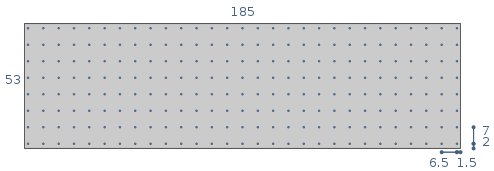
\includegraphics[width=.9\textwidth]{./figs/mh_dist.png}
\caption{Metal Halide luminaires distributed along the facility ceiling.}
\label{fig:mh_dist}
\end{figure}

\section{Calculus of Economy}

\subsection{Energy Consumption}
To calculate the energy consumption, the following data are needed:
\begin{itemize}
\item Number of luminaires: $232$
\item Energy cost: $0.093$\$
\item Electric demand cost: $11.00$\$
\item Number of hours per year: $16 \times 365.25 = 5,844$
\item Luminaire power: $458 W$
\end{itemize}
The numbers of hours per year assumes the leap year, so, the multiplier is $365.25$. The energy consumption results are showed as follow:
\begin{itemize}
\item Total power ($kW$): $232 \times 458 = 106,256 W = 106.256 kW$
\item Total electric demand cost per year: $11 \times 12 \times 106.256 = 14,025.79$\$
\item Total electric consumption cost per year: $5,844 \times 0.093 \times 106.256 = 57,749.29$\$
\item Total energy cost: $71,775.08$\$
\end{itemize}

\subsection{Average of Replaced Lamps per Year}
In order to calculate the average of lamps replaced per year, the following data are needed:
\begin{itemize}
\item Number of luminaires: $232$
\item Number of hours per year: $5,844$
\item Lamp lifetime hours at $80\%$ of survival: $14,000$
\end{itemize}

The Equation~\ref{eq:mh_relamp_average} shows the replaced lamps calculus.

\begin{equation}
\begin{split}
 & \text{Individual replaced lamps} \\
M_{individual} & = 20\% \times 232 \times \frac{5,844}{14,000} \\
 & = 19.37 \\
 & \approx 20
\end{split}
\begin{split}
 & \text{Collective replaced lamps} \\
M_{collective} & = 232 \times \frac {5,844}{14,000} \\
 & = 96.84 \\i
 & \approx 97
\end{split}
\label{eq:mh_relamp_average}
\end{equation}
Taking into account the worst case scenario, the calculation for this average is ceiling rounded. Thus, the average of replaced lamps per year is $117$.

\subsection{Relamping Workforce Cost per Year}
In order to calculate the cost for the relamping workforce per year, the following data are needed:
\begin{itemize}
\item Average of individual lamps replaced per year: $20$
\item Individual relamping cost: $87.00$\$
\item Average of collective luminaires replaced per year: $97$
\item Collective relamping cost: $9.00$\$
\end{itemize}

The average cost per year for the collective relamping is $873.00$\$ and for the individual relamping is $1,740,00$\$, so the total is $2.613,00$\$

              % chapitre 6
\chapter{High Pressure Sodium Luminaires}

The High Pressure Sodium (HPS) luminaire chosen is TH 400S PA22 (LEG = 8, SC = 1.4).

\section{Coefficient of Utilization}
The coefficient of utilization ($CU$) is calculated using the table given by the HPS luminaire~\cite{www:hps_photometric}. The calculus is demonstrated by the Equation~\ref{eq:hps_cu}.

\begin{equation*}
\begin{split}
\rho_c &= 70\%; \\
\rho_w &= 50\%; \\
\rho_f &= 20\%;
\end{split}
\qquad
\begin{split}
x &= 0.89; \\
x_1 &= 0; \\ y_1 &= 0.99 \\
x_2 &= 1; \\ y_2 &= 0.93
\end{split}
\qquad
\begin{split}
f(x) &= \frac{x_2 - x}{x_2 - x_1} \times y_1 +
       \frac{x - x_1}{x_2 - x_1} \times y_2 \\
 &= \frac{1 - 0.89}{1 - 0} \times 0.99 +
    \frac{0.89 - 0}{1 - 0} \times 0.93 \\
 & = 0.11 \times 0.99 - 0.89 \times 0.9 \\
 & = 0.909 \\
 & \approx 0.91
\end{split}
\label{eq:hps_cu_interpol_1}
\end{equation*}

\begin{equation*}
\begin{split}
\rho_c &= 50\%; \\
\rho_w &= 50\%; \\
\rho_f &= 20\%;
\end{split}
\qquad
\begin{split}
x &= 0.89; \\
x_1 &= 0; \\ y_1 &= 0.9 \\
x_2 &= 1; \\ y_2 &= 0.79
\end{split}
\qquad
\begin{split}
f(x) &= \frac{x_2 - x}{x_2 - x_1} \times y_1 +
       \frac{x - x_1}{x_2 - x_1} \times y_2 \\
 &= \frac{1 - 0.89}{1 - 0} \times 0.9 +
    \frac{0.89 - 0}{1 - 0} \times 0.79 \\
 & = 0.11 \times 0.9 - 0.89 \times 0.79 \\
 & = 0.802 \\
 & \approx 0.8
\end{split}
\label{eq:hps_cu_interpol_2}
\end{equation*}

\begin{equation}
\begin{split}
\rho_c &= 68.4\%; \\
\rho_w &= 50\%; \\
\rho_f &= 20\%;
\end{split}
\qquad
\begin{split}
x &= 68.4; \\
x_1 &= 50; \\ y_1 &= 0.79 \\
x_2 &= 70; \\ y_2 &= 0.91
\end{split}
\qquad
\begin{split}
f(x) &= \frac{x_2 - x}{x_2 - x_1} \times y_1 +
       \frac{x - x_1}{x_2 - x_1} \times y_2 \\
 &= \frac{70 - 68.4}{70 - 50} \times 0.79 +
    \frac{68.4 - 50}{70 - 50} \times 0.91 \\
 &= \frac{1.6}{20} \times 0.79 +
    \frac{18.4}{20} \times 0.91 \\
 & = 0.90 \\
CU_{hps} & = 0.90
\end{split}
\label{eq:hps_cu}
\end{equation}

\section{Light Loss Factor}
The light loss factor ($LLF$) is defined by the Equation~\ref{eq:LLF}.

\subsection{Lamp Lumen Depreciation}
The Equation~\ref{eq:hps_LLD} shows how to calculate the value of the $LLD$.

\begin{equation}
\begin{split}
LLD & = \frac{\text{Total downlight}}{\text{Design/Initial light}} \\
 & = \frac{33,853.5}{47,500} \\
 & =  0.713 \\
 & \approx 0.71
\end{split}
\label{eq:hps_LLD}
\end{equation}

\subsection{Luminaire Dirt Depreciation}
Following an operation time of 12 months between cleaning, and taking into account the facility environment with little windows and the use as a gymnasium, the environment, according to the new IES studies for LDD, has a moderate cleaning level. The HPS luminaire has the following characteristics:
\begin{itemize}
\item Luminaire semi-direct
\item Open class
\item Class XY
\item $LDD = 0.86$, according to the LDD factor graphic
\end{itemize}

\subsection{Ballast Efficacy}
The HPS ballast is a Constant Wattage Autotransformer (CWA) and according to a specification of a ballast like this~\cite{www:mh_hps_ballast}, its ballast factor is $1.0$.

\subsection{Calculating the LLF}
The Equation~\ref{eq:hps_LLF_calc} shows the calculus of the HPS's $LLF$.
\begin{equation}
\begin{split}
LLF &= 0.86 \times 0.71 \times 1.0 \\
    &= 0.61
\end{split}
\label{eq:hps_LLF_calc}
\end{equation}

\section{Number of Luminaires Calculus}
The amount of luminaires needed to achieve an illuminance of $500$ lux is calculated by the Equation~\ref{eq:hps_num_luminaires}.

\begin{equation}
\begin{split}
N_{lum} & = \frac{A_{total\,area} \times L_{Illuminance}}
                {N_{lumens} \times N_{lamps} \times CU \times LLF} \\
 & = \frac{9,805 \times 500}
          {47,500 \times 1 \times 0.9 \times 0.61} \\
 & = \frac{4,902,500}
          {26,103.15} \\
 & = 187.81 \\
 & \approx 188
\end{split}
\label{eq:hps_num_luminaires}
\end{equation}

The amount of luminaires to install is $189$, which gives a distribution of $27 \times 7$ and the spacing is calculated by the Equation~\ref{eq:hps_spacing}

\begin{equation}
\begin{split}
L: & \frac{185}
          {27} = 6.85\\
W: & \frac{53}
          {7} = 7.57
\end{split}
\qquad
\begin{split}
a & = 7 m \\
b & = 1.5 m \\
c & = 8 m \\
d & = 2.5 m
\end{split}
\label{eq:hps_spacing}
\end{equation}

The illuminance to be maintained for the installed luminaires is calculated by the Equation~\ref{eq:hps_maint_light}

\begin{equation}
\begin{split}
L_{Illuminance} & =
\frac {N_{lum} \times N_{lumens} \times N_{lamps} \times CU \times LLF}
      {A_{total\,area}} \\
 & = \frac{189 \times 47,500 \times 1 \times 0.9 \times 0.61}
          {9,805} \\
 & = 503.16 \\
 & \approx 503
\end{split}
\label{eq:hps_maint_light}
\end{equation}

\subsection{Checking the Spacing}
The Equation~\ref{eq:hps_shr} shows the calculus to check the spacing height ratio ($SHR$) attends the spacing criterion ($SC$).

\begin{equation}
\begin{split}
SHR & = \frac {1}{HM} \times \sqrt{\frac{A_{total\,area}}{N_{lum}}} \\
 & = \frac {1}{7.5} \times \sqrt{\frac{9,805}{189}} \\
 & = 0.133 \times \sqrt{51.88} \\
 & = 0.133 \times 7.2 \\
 & = 0.96 \\
\end{split}
\label{eq:hps_shr}
\end{equation}

The $SC$ given by the HPS luminaire~\cite{www:hps_photometric} is $1.4$ and the $SHR$ has an acceptable value when $SHR \leq SC$, thus the obtained $SHR$ is good.

\section{Luminaires Distribution}
The distribution of the luminaires is represented on Figure~\ref{fig:hps_dist}.
\begin{figure}[h!]
\centering
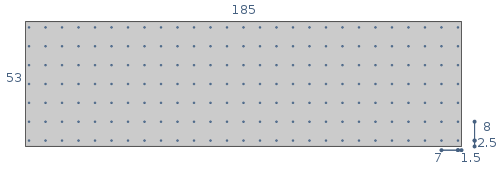
\includegraphics[width=.9\textwidth]{./figs/hps_dist.png}
\caption{High Pressure Sodium luminaires distributed along the facility ceiling.}
\label{fig:hps_dist}
\end{figure}

\section{Calculus of Economy}

\subsection{Energy Consumption}
To calculate the energy consumption, the following data are needed:
\begin{itemize}
\item Number of luminaires: $189$
\item Energy cost: $0.093$\$
\item Electric demand cost: $11.00$\$
\item Number of hours per year: $16 \times 365.25 = 5,844$
\item Luminaire power: $465 W$
\end{itemize}
The numbers of hours per year assumes the leap year, so, the multiplier is $365.25$. The energy consumption results are showed as follow:
\begin{itemize}
\item Total power ($kW$): $189 \times 465 = 87,885 W = 87.885 kW$
\item Total electric demand cost per year: $11 \times 12 \times 87.885 = 11,600.82$\$
\item Total electric consumption cost per year: $5,844 \times 0.093 \times 87.885 = 47,764.79$\$
\item Total energy cost: $59,365.61$\$
\end{itemize}

\subsection{Average of Replaced Lamps per Year}
In order to calculate the average of lamps replaced per year, the following data are needed:
\begin{itemize}
\item Number of luminaires: $189$
\item Number of hours per year: $5,844$
\item Lamp lifetime hours at $80\%$ of survival: $19,200$
\end{itemize}

The Equation~\ref{eq:hps_relamp_average} shows the replaced lamps calculus.

\begin{equation}
\begin{split}
 & \text{Individual replaced lamps} \\
M_{individual} & = 20\% \times 189 \times \frac{5,844}{19,200} \\
 & = 11.51 \\
 & \approx 12
\end{split}
\begin{split}
 & \text{Collective replaced lamps} \\
M_{collective} & = 189 \times \frac {5,844}{19.200} \\
 & = 57.53 \\
 & \approx 58
\end{split}
\label{eq:hps_relamp_average}
\end{equation}
Taking into account the worst case scenario, the calculation for this average is ceiling rounded. Thus, the average of replaced lamps per year is $70$.

\subsection{Relamping Workforce Cost per Year}
In order to calculate the cost for the relamping workforce per year, the following data are needed:
\begin{itemize}
\item Average of individual lamps replaced per year: $12$
\item Individual relamping cost: $87.00$\$
\item Average of collective luminaires replaced per year: $58$
\item Collective relamping cost: $9.00$\$
\end{itemize}

The average cost per year for the collective relamping is $522.00$\$ and for the individual relamping is $1,044,00$\$, so the total is $1.566,00$\$

              % chapitre 7
\chapter{Point by Point Method}

The point by point method will be applied to the HPS lamp. The candela table is presented in the Table~\ref{tab:hps_candela}.

\begin{table}
\centering
\begin{tabular}{|l|r|}
  \hline
  \textbf{Angle} & \textbf{Candela} \\
  \hline
  0 & 12984 \\
  \hline
  5 & 13072 \\
  \hline
  15 & 12892 \\
  \hline
  25 & 13402 \\
  \hline
  35 & 13033 \\
  \hline
  45 & 8792 \\
  \hline
  55 & 3584 \\
  \hline
  65 & 1355 \\
  \hline
  75 & 1379 \\
  \hline
  85 & 1572 \\
  \hline
  90 & 1638 \\
  \hline
  95 & 1686 \\
  \hline
  105 & 1721 \\
  \hline
  115 & 1682 \\
  \hline
  125 & 1560 \\
  \hline
  135 & 1416 \\
  \hline
  145 & 1361 \\
  \hline
  155 & 1042 \\
  \hline
  165 & 676 \\
  \hline
  175 & 339 \\
  \hline
  180 & 0 \\
  \hline
\end{tabular}
\caption{Candela table for the luminaire TH 400S PA22 (LEG 8, SC= 1.4).}
\label{tab:hps_candela}
\end{table}

\section{Lux Meter positioned under the luminaire}
Based on the candela Table~\ref{tab:hps_candela} and the Figure~\ref{fig:pp_under_lum}, the calculation of the illuminance for the groups of luminaires is presented by the Equations~\cref{eq:pp_under_point_a,eq:pp_under_point_b,eq:pp_under_point_c,eq:pp_under_point_d,eq:pp_under_point_e,eq:pp_under_point_f,eq:pp_under_lum}.

\begin{figure}[h!]
\centering
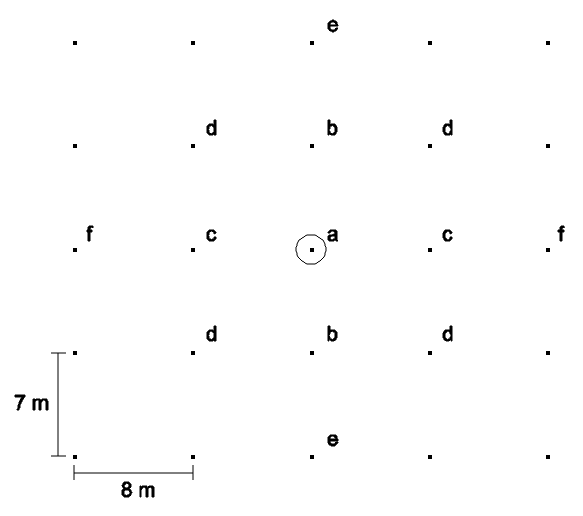
\includegraphics[width=.5\textwidth]{./figs/pp_under_lum.png}
\caption{Point by point method when the lux meter is under one luminaire.}
\label{fig:pp_under_lum}
\end{figure}

The Equation~\ref{eq:pp_under_point_a} presents the calculation for the point $a$.
\begin{equation}
\begin{split}
I_a &= \frac{I_{(cd)} \times \cos^3(\theta)}{H^2} \\
 &= \frac{12,984 \times \cos^3(0\degree)}{7.5^2} \\
 &= \frac{12,984}{56.25} \\
 & = 230.827 \\
 & \approx 230.83 lux
\end{split}
\label{eq:pp_under_point_a}
\end{equation}

The Equation~\ref{eq:pp_under_point_b} presents the calculation for the point $b$.
\begin{equation}
\begin{split}
\theta &= \tan^{-1}\left( \frac{Opposite}{Adjacent} \right) \\
 & = \tan^{-1}\left( \frac{7}{7.5} \right) \\
 & = 43.03\degree \\
 & \approx 43\degree\\
\\
x & = 43 \\
x_1 & = 35 \quad y_1 = 13,033 \\
x_2 & = 45 \quad y_2 = 8,792 \\
f(x) &= \frac{x_2 - x}{x_2 - x_1} \times y_1 +
       \frac{x - x_1}{x_2 - x_1} \times y_2 \\
 &= \frac{45 - 43}{45 - 35} \times 13,033 +
    \frac{43 - 35}{45 - 35} \times 8,792 \\
 & = 0.2 \times 13,033 - 0.8 \times 8,792 \\
 & = 9,632.2\: cd \\
\\
I_b &= \frac{I_{(cd)} \times \cos^3(\theta)}{H^2} \\
 &= \frac{9,632 \times \cos^3(43\degree)}{7.5^2} \\
 &= \frac{9,632 \times 0.39}{56.25} \\
 & = 66.986 \\
 & \approx 66.99\: lux
\end{split}
\label{eq:pp_under_point_b}
\end{equation}

The Equation~\ref{eq:pp_under_point_c} presents the calculation for the point $c$.
\begin{equation}
\begin{split}
\theta &= \tan^{-1}\left( \frac{Opposite}{Adjacent} \right) \\
 & = \tan^{-1}\left( \frac{8}{7.5} \right) \\
 & = 46.847\degree \\
 & \approx 47\degree\\
\\
x & = 47 \\
x_1 & = 45 \quad y_1 = 8,792 \\
x_2 & = 55 \quad y_2 = 3,584 \\
f(x) &= \frac{x_2 - x}{x_2 - x_1} \times y_1 +
       \frac{x - x_1}{x_2 - x_1} \times y_2 \\
 &= \frac{55 - 47}{55 - 45} \times 8,792 +
    \frac{47 - 45}{55 - 45} \times 3,584 \\
 & = 0.8 \times 8,792 - 0.2 \times 3,584 \\
 & = 7,750.4\: cd \\
\\
I_c &= \frac{I_{(cd)} \times \cos^3(\theta)}{H^2} \\
 &= \frac{7,750 \times \cos^3(47\degree)}{7.5^2} \\
 &= \frac{7,750 \times 0.31}{56.25} \\
 & = 43.707 \\
 & \approx 43.71\: lux
\end{split}
\label{eq:pp_under_point_c}
\end{equation}

The Equation~\ref{eq:pp_under_point_d} presents the calculation for the point $d$.
\begin{equation}
\begin{split}
s_{distance} & = \sqrt{8^2 + 7^2} \\
 & = \sqrt{113} \\
 & = 10.63 \\
\\
\theta &= \tan^{-1}\left( \frac{Opposite}{Adjacent} \right) \\
 & = \tan^{-1}\left( \frac{10.63}{7.5} \right) \\
 & = 54.795\degree \\
 & \approx 55\degree\\
\\
I_d &= \frac{I_{(cd)} \times \cos^3(\theta)}{H^2} \\
 &= \frac{3,584 \times \cos^3(55\degree)}{7.5^2} \\
 &= \frac{3,584 \times 0.19}{56.25} \\
 & = 12.023 \\
 & \approx 12.02\: lux
\end{split}
\label{eq:pp_under_point_d}
\end{equation}

The Equation~\ref{eq:pp_under_point_e} presents the calculation for the point $e$.
\begin{equation}
\begin{split}
s_{distance} = 14\\
\theta &= \tan^{-1}\left( \frac{Opposite}{Adjacent} \right) \\
 & = \tan^{-1}\left( \frac{14}{7.5} \right) \\
 & = 61.82\degree \\
 & \approx 62\degree\\
\\
x & = 62 \\
x_1 & = 55 \quad y_1 = 3,584 \\
x_2 & = 65 \quad y_2 =  1,355 \\
f(x) &= \frac{x_2 - x}{x_2 - x_1} \times y_1 +
       \frac{x - x_1}{x_2 - x_1} \times y_2 \\
 &= \frac{65 - 62}{65 - 55} \times 3,584 +
    \frac{62 - 55}{65 - 55} \times 1,355 \\
 & = 0.3 \times 3,584 - 0.7 \times 1,355 \\
 & = 2,023.7\: cd \\
\\
I_e &= \frac{I_{(cd)} \times \cos^3(\theta)}{H^2} \\
 &= \frac{2,023.7 \times \cos^3(62\degree)}{7.5^2} \\
 &= \frac{2,023.7 \times 0.104}{56.25} \\
 & = 3.723 \\
 & \approx 3.72\: lux
\end{split}
\label{eq:pp_under_point_e}
\end{equation}

The Equation~\ref{eq:pp_under_point_f} presents the calculation for the point $f$.
\begin{equation}
\begin{split}
s_{distance} = 16\\
\theta &= \tan^{-1}\left( \frac{Opposite}{Adjacent} \right) \\
 & = \tan^{-1}\left( \frac{16}{7.5} \right) \\
 & = 64.885\degree \\
 & \approx 65\degree\\
\\
I_f &= \frac{I_{(cd)} \times \cos^3(\theta)}{H^2} \\
 &= \frac{1,355 \times \cos^3(65\degree)}{7.5^2} \\
 &= \frac{1,355 \times 0.075}{56.25} \\
 & = 1.818 \\
 & \approx 1.82\: lux
\end{split}
\label{eq:pp_under_point_f}
\end{equation}

The Equation~\ref{eq:pp_under_lum} presents the calculation for the total illumination contribution.
\begin{equation}
\begin{split}
I_{total} &= I_a + 2 \times I_b + 2 \times I_c + 4 \times I_d + 2 \times I_e + 2 \times I_f \\
 &= 230.83 + 2 \times 66.99 + 2 \times 43.71 + 4 \times 12.02 + 2 \times 3.72 + 2 \times 1.82 \\
 & = 511.39 \\
\end{split}
\label{eq:pp_under_lum}
\end{equation}

\section{Lux Meter positioned between two luminaires}
Based on the candela Table~\ref{tab:hps_candela} and the Figure~\ref{fig:pp_between_2_lum}, the calculation of the illuminance for the groups of luminaires is presented by the Equations~\cref{eq:pp_between_2_point_a,eq:pp_between_2_point_b,eq:pp_between_2_point_c,eq:pp_between_2_point_d,eq:pp_between_2_point_e,eq:pp_between_2_point_f,eq:pp_between_2_lum}.

\begin{figure}[h!]
\centering
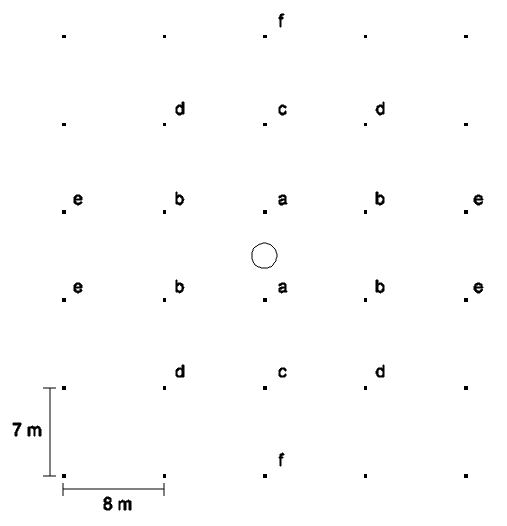
\includegraphics[width=.5\textwidth]{./figs/pp_between_2_lum.png}
\caption{Point by point method when the lux meter is between two luminaires.}
\label{fig:pp_between_2_lum}
\end{figure}

The Equation~\ref{eq:pp_between_2_point_a} presents the calculation for the point $a$.
\begin{equation}
\begin{split}
s_{distance} = 3.5\\
\theta &= \tan^{-1}\left( \frac{Opposite}{Adjacent} \right) \\
 & = \tan^{-1}\left( \frac{3.5}{7.5} \right) \\
 & = 25.16\degree \\
 & \approx 25\degree\\
\\
I_a &= \frac{I_{(cd)} \times \cos^3(\theta)}{H^2} \\
 &= \frac{13,402 \times \cos^3(25\degree)}{7.5^2} \\
 &= \frac{13,402 \times 0.74}{56.25} \\
 & = 177.368 \\
 & \approx 177.37 lux
\end{split}
\label{eq:pp_between_2_point_a}
\end{equation}

The Equation~\ref{eq:pp_between_2_point_b} presents the calculation for the point $b$.
\begin{equation}
\begin{split}
s_{distance} & = \sqrt{3.5^2 + 8^2} \\
 & = \sqrt{76.25} \\
 & = 8.73 \\
\\
\theta &= \tan^{-1}\left( \frac{Opposite}{Adjacent} \right) \\
 & = \tan^{-1}\left( \frac{8.73}{7.5} \right) \\
 & = 49.334\degree \\
 & \approx 49\degree\\
\\
x & = 49 \\
x_1 & = 45 \quad y_1 = 8,792 \\
x_2 & = 55 \quad y_2 = 3,584 \\
f(x) &= \frac{x_2 - x}{x_2 - x_1} \times y_1 +
       \frac{x - x_1}{x_2 - x_1} \times y_2 \\
 &= \frac{55 - 49}{55 - 45} \times 8,792 +
    \frac{49 - 45}{55 - 45} \times 3,584 \\
 & = 0.6 \times 8,792 - 0.4 \times 3,584 \\
 & = 6,708.8\: cd \\
\\
I_b &= \frac{I_{(cd)} \times \cos^3(\theta)}{H^2} \\
 &= \frac{6,708.8 \times \cos^3(49\degree)}{7.5^2} \\
 &= \frac{6,708.8 \times 0.28}{56.25} \\
 & = 33.678 \\
 & \approx 33.68\: lux
\end{split}
\label{eq:pp_between_2_point_b}
\end{equation}

The Equation~\ref{eq:pp_between_2_point_c} presents the calculation for the point $c$.
\begin{equation}
\begin{split}
s_{distance} = 10.5\\
\theta &= \tan^{-1}\left( \frac{Opposite}{Adjacent} \right) \\
 & = \tan^{-1}\left( \frac{10.5}{7.5} \right) \\
 & = 54.46\degree \\
 & \approx 55\degree\\
\\
I_c &= \frac{I_{(cd)} \times \cos^3(\theta)}{H^2} \\
 &= \frac{3,584 \times \cos^3(55\degree)}{7.5^2} \\
 &= \frac{3,584 \times 0.19}{56.25} \\
 & = 12.023 \\
 & \approx 12.023\: lux
\end{split}
\label{eq:pp_between_2_point_c}
\end{equation}

The Equation~\ref{eq:pp_between_2_point_d} presents the calculation for the point $d$.
\begin{equation}
\begin{split}
s_{distance} & = \sqrt{10.5^2 + 8^2} \\
 & = \sqrt{174.25} \\
 & = 13.2 \\
\\
\theta &= \tan^{-1}\left( \frac{Opposite}{Adjacent} \right) \\
 & = \tan^{-1}\left( \frac{12.2}{7.5} \right) \\
 & = 60.396\degree \\
 & \approx 60\degree\\
\\
x & = 60 \\
x_1 & = 55 \quad y_1 = 3,584 \\
x_2 & = 65 \quad y_2 = 1,355 \\
f(x) &= \frac{x_2 - x}{x_2 - x_1} \times y_1 +
       \frac{x - x_1}{x_2 - x_1} \times y_2 \\
 &= \frac{65 - 60}{65 - 55} \times 3,584 +
    \frac{60 - 55}{65 - 55} \times 1,355 \\
 & = 0.5 \times 3,584 - 0.5 \times 1,355 \\
 & = 2,469.5\: cd \\
\\
I_d &= \frac{I_{(cd)} \times \cos^3(\theta)}{H^2} \\
 &= \frac{2,469.5 \times \cos^3(60\degree)}{7.5^2} \\
 &= \frac{2,469.5 \times 0.125}{56.25} \\
 & = 5.488 \\
 & \approx 5.49\: lux
\end{split}
\label{eq:pp_between_2_point_d}
\end{equation}

The Equation~\ref{eq:pp_between_2_point_e} presents the calculation for the point $e$.
\begin{equation}
\begin{split}
s_{distance} & = \sqrt{3.5^2 + 16^2} \\
 & = \sqrt{268.25} \\
 & = 16.38 \\
\theta &= \tan^{-1}\left( \frac{Opposite}{Adjacent} \right) \\
 & = \tan^{-1}\left( \frac{16.38}{7.5} \right) \\
 & = 65.398\degree \\
 & \approx 65\degree\\
\\
I_e &= \frac{I_{(cd)} \times \cos^3(\theta)}{H^2} \\
 &= \frac{1,355 \times \cos^3(65\degree)}{7.5^2} \\
 &= \frac{1,355 \times 0.075}{56.25} \\
 & = 1.818 \\
 & \approx 1.82\: lux
\end{split}
\label{eq:pp_between_2_point_e}
\end{equation}

The Equation~\ref{eq:pp_between_2_point_f} presents the calculation for the point $f$.
\begin{equation}
\begin{split}
s_{distance} = 17.5\\
\theta &= \tan^{-1}\left( \frac{Opposite}{Adjacent} \right) \\
 & = \tan^{-1}\left( \frac{17.5}{7.5} \right) \\
 & = 66.801\degree \\
 & \approx 67\degree\\
\\
x & = 67 \\
x_1 & = 65 \quad y_1 = 1,355 \\
x_2 & = 75 \quad y_2 = 1,379 \\
f(x) &= \frac{x_2 - x}{x_2 - x_1} \times y_1 +
       \frac{x - x_1}{x_2 - x_1} \times y_2 \\
 &= \frac{75 - 67}{75 - 65} \times 1,355 +
    \frac{67 - 65}{75 - 65} \times 1,379 \\
 & = 0.8 \times 1,355 - 0.2 \times 1,379 \\
 & = 1,359.8\: cd \\
\\
I_f &= \frac{I_{(cd)} \times \cos^3(\theta)}{H^2} \\
 &= \frac{1,359.8 \times \cos^3(67\degree)}{7.5^2} \\
 &= \frac{1,359.8 \times 0.06}{56.25} \\
 & = 1.442 \\
 & \approx 1.44\: lux
\end{split}
\label{eq:pp_between_2_point_f}
\end{equation}

The Equation~\ref{eq:pp_between_2_lum} presents the calculation for the total illumination contribution.
\begin{equation}
\begin{split}
I_{total} &= 2 \times I_a + 4 \times I_b + 2 \times I_c + 4 \times I_d + 4 \times I_e + 2 \times I_f \\
 &= 2 \times 177.37 + 4 \times 33.68 + 2 \times 12.02 + 4 \times 5.49 + 4 \times 1.82 + 2 \times 1.44 \\
 & = 545.62 \\
\end{split}
\label{eq:pp_between_2_lum}
\end{equation}

\section{Lux Meter positioned between four luminaires}
Based on the candela Table~\ref{tab:hps_candela} and the Figure~\ref{fig:pp_between_4_lum}, the calculation of the illuminance for the groups of luminaires is presented by the Equations~\cref{eq:pp_between_4_point_a,eq:pp_between_4_point_b,eq:pp_between_4_point_c,eq:pp_between_4_point_d,eq:pp_between_4_point_e,eq:pp_between_4_lum}.

\begin{figure}[h!]
\centering
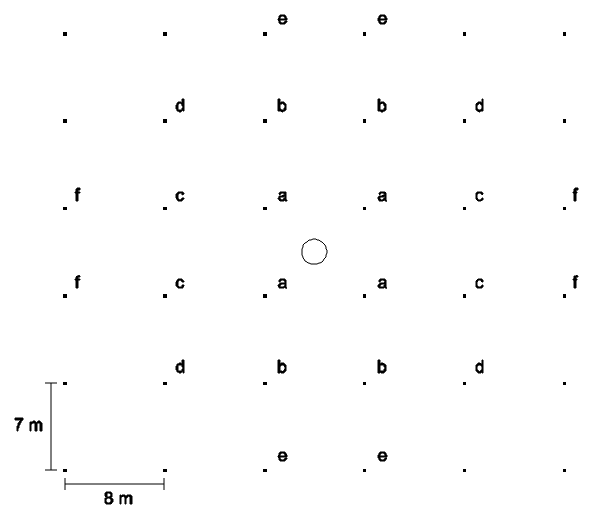
\includegraphics[width=.5\textwidth]{./figs/pp_between_4_lum.png}
\caption{Point by point method when the lux meter is between four luminaires.}
\label{fig:pp_between_4_lum}
\end{figure}

The Equation~\ref{eq:pp_between_4_point_a} presents the calculation for the point $a$.
\begin{equation}
\begin{split}
s_{distance} & = \sqrt{3.5^2 + 4^2} \\
 & = \sqrt{28.25} \\
 & = 5.32 \\
\theta &= \tan^{-1}\left( \frac{Opposite}{Adjacent} \right) \\
 & = \tan^{-1}\left( \frac{5.32}{7.5} \right) \\
 & = 35.349\degree \\
 & \approx 35\degree\\
\\
I_a &= \frac{I_{(cd)} \times \cos^3(\theta)}{H^2} \\
 &= \frac{13,033 \times \cos^3(35\degree)}{7.5^2} \\
 &= \frac{13,033 \times 0.55}{56.25} \\
 & = 127.355 \\
 & \approx 127.36 lux
\end{split}
\label{eq:pp_between_4_point_a}
\end{equation}

The Equation~\ref{eq:pp_between_4_point_b} presents the calculation for the point $b$.
\begin{equation}
\begin{split}
s_{distance} & = \sqrt{3.5^2 + 10.5^2} \\
 & = \sqrt{122.25} \\
 & = 11.07 \\
\\
\theta &= \tan^{-1}\left( \frac{Opposite}{Adjacent} \right) \\
 & = \tan^{-1}\left( \frac{10.07}{7.5} \right) \\
 & = 55.88\degree \\
 & \approx 56\degree\\
\\
x & = 56 \\
x_1 & = 55 \quad y_1 = 3,584 \\
x_2 & = 65 \quad y_2 = 1,355 \\
f(x) &= \frac{x_2 - x}{x_2 - x_1} \times y_1 +
       \frac{x - x_1}{x_2 - x_1} \times y_2 \\
 &= \frac{65 - 56}{65 - 55} \times 3,584 +
    \frac{56 - 55}{65 - 55} \times 1,355 \\
 & = 0.9 \times 3,584 - 0.1 \times 1,355 \\
 & = 3,361.1\: cd \\
\\
I_b &= \frac{I_{(cd)} \times \cos^3(\theta)}{H^2} \\
 &= \frac{3,361.1 \times \cos^3(56\degree)}{7.5^2} \\
 &= \frac{3,361.1 \times 0.17}{56.25} \\
 & = 10.448 \\
 & \approx 10.45\: lux
\end{split}
\label{eq:pp_between_4_point_b}
\end{equation}

The Equation~\ref{eq:pp_between_4_point_c} presents the calculation for the point $c$.
\begin{equation}
\begin{split}
s_{distance} & = \sqrt{3.5^2 + 12^2} \\
 & = \sqrt{156.25} \\
 & = 12.5 \\
\\
\theta &= \tan^{-1}\left( \frac{Opposite}{Adjacent} \right) \\
 & = \tan^{-1}\left( \frac{12.5}{7.5} \right) \\
 & = 59.04\degree \\
 & \approx 59\degree\\
\\
x & = 59 \\
x_1 & = 55 \quad y_1 = 3,584 \\
x_2 & = 65 \quad y_2 = 1,355 \\
f(x) &= \frac{x_2 - x}{x_2 - x_1} \times y_1 +
       \frac{x - x_1}{x_2 - x_1} \times y_2 \\
 &= \frac{65 - 59}{65 - 55} \times 3,584 +
    \frac{59 - 55}{65 - 55} \times 1,355 \\
 & = 0.6 \times 3,584 - 0.4 \times 1,355 \\
 & = 2,692.4\: cd \\
\\
I_c &= \frac{I_{(cd)} \times \cos^3(\theta)}{H^2} \\
 &= \frac{2,692.4 \times \cos^3(59\degree)}{7.5^2} \\
 &= \frac{2,692.4 \times 0.14}{56.25} \\
 & = 6.539 \\
 & \approx 6.54\: lux
\end{split}
\label{eq:pp_between_4_point_c}
\end{equation}

The Equation~\ref{eq:pp_between_4_point_d} presents the calculation for the point $d$.
\begin{equation}
\begin{split}
s_{distance} & = \sqrt{10.5^2 + 12^2} \\
 & = \sqrt{254.25} \\
 & = 15.95 \\
\\
\theta &= \tan^{-1}\left( \frac{Opposite}{Adjacent} \right) \\
 & = \tan^{-1}\left( \frac{15.95}{7.5} \right) \\
 & = 64.816\degree \\
 & \approx 65\degree\\
\\
I_d &= \frac{I_{(cd)} \times \cos^3(\theta)}{H^2} \\
 &= \frac{1,355 \times \cos^3(65\degree)}{7.5^2} \\
 &= \frac{1,355 \times 0.075}{56.25} \\
 & = 1.818 \\
 & \approx 1.82\: lux
\end{split}
\label{eq:pp_between_4_point_d}
\end{equation}

The Equation~\ref{eq:pp_between_4_point_e} presents the calculation for the point $e$.
\begin{equation}
\begin{split}
s_{distance} & = \sqrt{3.5^2 + 17.5^2} \\
 & = \sqrt{318.25} \\
 & = 17.85 \\
\theta &= \tan^{-1}\left( \frac{Opposite}{Adjacent} \right) \\
 & = \tan^{-1}\left( \frac{17.85}{7.5} \right) \\
 & = 67.209\degree \\
 & \approx 67\degree\\
\\
x & = 67 \\
x_1 & = 65 \quad y_1 = 1,355 \\
x_2 & = 75 \quad y_2 = 1,379 \\
f(x) &= \frac{x_2 - x}{x_2 - x_1} \times y_1 +
       \frac{x - x_1}{x_2 - x_1} \times y_2 \\
 &= \frac{75 - 67}{75 - 65} \times 1,355 +
    \frac{67 - 65}{75 - 65} \times 1,379 \\
 & = 0.8 \times 1,355 - 0.2 \times 1,379 \\
 & = 1,359.8\: cd \\
\\
I_e &= \frac{I_{(cd)} \times \cos^3(\theta)}{H^2} \\
 &= \frac{1,359.8 \times \cos^3(67\degree)}{7.5^2} \\
 &= \frac{1,359.8 \times 0.06}{56.25} \\
 & = 1.442 \\
 & \approx 1.44\: lux
\end{split}
\label{eq:pp_between_4_point_e}
\end{equation}

The Equation~\ref{eq:pp_between_4_lum} presents the calculation for the total illumination contribution.
\begin{equation}
\begin{split}
I_{total} &= 4 \times I_a + 4 \times I_b + 4 \times I_c + 4 \times I_d + 4 \times I_e \\
 &= 4 \times 127.36 + 4 \times 10.45 + 4 \times 6.54 + 4 \times 1.82 + 4 \times 1.44 \\
 & = 590.44 \\
\end{split}
\label{eq:pp_between_4_lum}
\end{equation}

\section{Uniformity Test}
The Equation~\ref{eq:test_unif} presents the uniformity test calculation.
\begin{equation}
\begin{split}
T &= \frac{I_{bigger\,value} - I_{lower\,value}}{I_{lower\,value}} \\
 &= \frac{590.44 - 511.39}{511.39} \\
 & = 0.1546 \\
 & \approx 15.46\%
\end{split}
\label{eq:test_unif}
\end{equation}
The result of the Equation~\ref{eq:test_unif} shows that this project has uniformity, because the test is lower than $30\%$.



              % chapitre 8

\appendix                       % annexes le cas échéant

\chapter{Lamps and Luminaires Prices}

The prices of all luminaires were quoted by AMP~\cite{www:luminaires_saler}, as well as the led board (led lamp).

The fluorescent lamps were found for sale at~\cite{www:fluo_lamp_saler}, the MH lamps at~\cite{www:mh_lamp_saler} and HPS lamps at~\cite{www:hps_lamp_saler}.

              % annexe A

\bibliography{lighting_work}    % production de la bibliographie

\end{document}
